\documentclass{standalone}

\usepackage{tikz}
\usepackage{amsmath}
\usetikzlibrary{math}

% definition of all the colors
\usepackage{xcolor}
%
% genertated by ./compile.py
%

\definecolor{codegreen}{RGB}{0, 153, 0}
\definecolor{codegray}{RGB}{127, 127, 127}
\definecolor{codeblue}{RGB}{102, 214, 237}
\definecolor{codekeyword}{RGB}{249, 36, 114}
\definecolor{codecomment}{RGB}{127, 127, 127}
\definecolor{backcolor}{RGB}{242, 242, 235}
\definecolor{linkcolor}{RGB}{102, 0, 0}
\definecolor{corange}{RGB}{255, 70, 0}
\definecolor{cyellow}{RGB}{209, 153, 0}
\definecolor{cblue}{RGB}{64, 128, 255}
\definecolor{cbrown}{RGB}{153, 102, 51}
\definecolor{cpink}{RGB}{255, 0, 255}
\definecolor{cred}{RGB}{255, 64, 0}
\definecolor{cgreen}{RGB}{0, 191, 0}
\definecolor{clightblue}{RGB}{191, 217, 255}
\definecolor{cturquois}{RGB}{0, 255, 255}
\definecolor{cpurple}{RGB}{128, 0, 255}
\definecolor{clightgreen}{RGB}{175, 255, 175}
\definecolor{clightpink}{RGB}{255, 175, 255}
\definecolor{cdarkblue}{RGB}{0, 0, 255}
\definecolor{cdarkred}{RGB}{255, 0, 0}
\definecolor{cdarkgreen}{RGB}{0, 255, 0}


\begin{document}

%\tikzset{every picture/.style={line width=0.75pt}} %set default line width to 0.75pt        

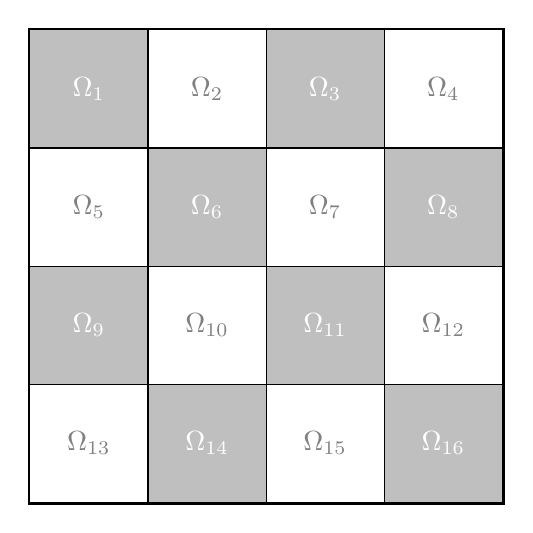
\begin{tikzpicture}[]

\def\i{1}
\def\step{1.5}
\def\width{4}
\def\height{4}

\pgfmathsetmacro\tx{\width*\step}
\pgfmathsetmacro\ty{\height*\step}
\draw[black, ultra thick] (0,0) rectangle (\tx,\ty); % full rectangle

\foreach \y in {\height,...,1} {
	\pgfmathsetmacro\ye{\y*\step}
	\pgfmathsetmacro\ys{(\y - 1)*\step}
	\foreach \x in {1,...,\width} {
		\pgfmathsetmacro\xs{(\x - 1)*\step}
		\pgfmathsetmacro\xe{\x*\step}
		\pgfmathtruncatemacro{\j}{mod(\x+\y,2)}
		\ifnum \j=1
			\draw[black, thin, fill=lightgray ] ((\xs,\ys) rectangle (\xe,\ye) node[pos=.5] {\textcolor{white}{$\Omega_{\i}$}};
		\else
			\draw[black, thin, fill=white] ((\xs,\ys) rectangle (\xe,\ye) node[pos=.5] {\textcolor{gray}{$\Omega_{\i}$} };
		\fi
		\pgfmathparse{int(\i+1)}
		\xdef\i{\pgfmathresult}
	}
}

%\draw[black, ultra thick] (0,0) rectangle (9,9); % full rectangle

%\draw[black, thin] (0,0) 			 rectangle (\step,\step) 	 node[pos=.5] {$\Omega_7$};
%\draw[black, thin] (\step,0) 		 rectangle (\step*2,\step) 	 node[pos=.5] {$\Omega_8$};
%\draw[black, thin] (\step*2,0) 		 rectangle (\step*3,\step) 	 node[pos=.5] {$\Omega_9$};

%\draw[black, thin] (0,\step) 		 rectangle (\step,\step*2) 	 node[pos=.5] {$\Omega_4$};
%\draw[black, thin] (\step,\step) 	 rectangle (\step*2,\step*2) node[pos=.5] {$\Omega_5$};
%\draw[black, thin] (\step*2,\step) 	 rectangle (\step*3,\step*2) node[pos=.5] {$\Omega_6$};

%\draw[black, thin] (0,\step*2) 		 rectangle (\step,\step*3)   node[pos=.5] {$\Omega_1$};
%\draw[black, thin] (\step,\step*2) 	 rectangle (\step*2,\step*3) node[pos=.5] {$\Omega_2$};
%\draw[black, thin] (\step*2,\step*2) rectangle (\step*3,\step*3) node[pos=.5] {$\Omega_3$};


\end{tikzpicture}


\end{document}